\section{Implementation}
\label{Implementation section}
As was stated in the introduction, we have two main implementations: 
\subsection*{Simplistic Python implementation}
The Python implementation uses simplistic quadcopter dynamics only defined by:
\begin{itemize}
    \item Quad mass: $m_b$
    \item Moments of inertia: $I_{xx}$, $I_{yy}$, $I_{zz}$
    \item drag coefficient: $A_{x}$, $A_{y}$, $A_{z}$
    \item pd attitude gains: $K_{\phi_{p}}$, $K_{\phi_{d}}$, $K_{\psi_{p}}$, $K_{\psi_{d}}$, $K_{\theta_{p}}$, $K_{\theta_{d}}$
\end{itemize}

We use ODEint to evolve the state of the system by doing to following on each iteration: 
\begin{itemize}
    \item First we compute the current Mass Matrix $M$, Coriolis Matrix $C$, Control Matrix $B$, gravity Matrix $G$
    \item Then we pass to the PVFC controller those dynamics together with the desired velocity field and compute a desired thurst vector according to (cite pvfc equations)
    \item For a given desired thrust vector, The quad uses a simple attitude PD control law to compute the state derivates of the quad
\end{itemize}


The desired velocity fields are computed using Sympy (A Python library for symbolic ) for easy field and field gradient computation. Since most fields we used are derived from potential functions, we can easily obtain the field and field jacobian required by PVFC by symbolically differentiating their potentials or shaping functions.

\subsection*{Full Sensor Placement pipeline in ROS/Gazebo/PX4}
In this implementation, we are using a real world quadrotor called IRIS quad provided in the PX4 SITL package. 
The dynamics are evolved and computed by Gazebo. 
The implementation is divided in 2 ROS Nodes, 1 ROS-PCL Node, 1 Gazebo-ROS plugin, and 1 PX4/MAVROS node:
\begin{itemize}
    \item Velocity Field ROS Node: This node subscribe to the mavros odometry topic, computes the velocity Field at the current position and publishes the desired field and field gradient. 
    We implemented all the velocity field using the symbolic math library SymEngine so that all gradient computations from potential or shaping function would be done automatically. 
    In addition, this node is implementing a state machine such that in each state, a specific field is being used.
    Specifically, the first state gives a sink to get altitude, the second state is a sink field to approach the target, 
    the third state represents the contact phase with the wall(the node subscribes to a topic called "grasping" to know if the grasping arm is currently activated) it starts when an engagement signal is received from the grasping arm and it finishes when a disengagment signal is received from the grasping arm. 
    The last state is to get away from the wall and land, we use a sink field to implement it.
    We implemented an obstacle avoidance system for generic superquadratic obstacles, upon obstacle detection, we compute the avoidance field for this obstacle from the appropriate shaping function, an irrotational field is generated to avoid the obstacle. This node subscribes to an obstacle topic to know when new obstacle have been detected. 
    \item PVFC ROS Node: This node  subscribes to the desired velocity field and to the MAVROS odometry and publishes a thurst vector on the MAVROS attitude topic computed my the PVFC controller.
    \item MAVROS Node :This node is the interface between the PX4 firmware and ROS
    \item PCL Object Segmentation Node: This node reuses the code of a PCL tutorial performing cylinder segmentation on point cloud data(cite). We added a ROS integration to to the velocity field topic the position of the detected object and also we implemented the transforms from camera point of view to FCU frame, and from FCU frame to world frame. 
    \item Grasping arm Gazebo-ROS plugin: This node reuses the code of the vaccuum arm of Gazebo, but it was modified so that could be "attached" to the moving IRIS model and attach to a wall in Gazebo. 
\end{itemize}

\begin{figure*}[h!]
    \centering
    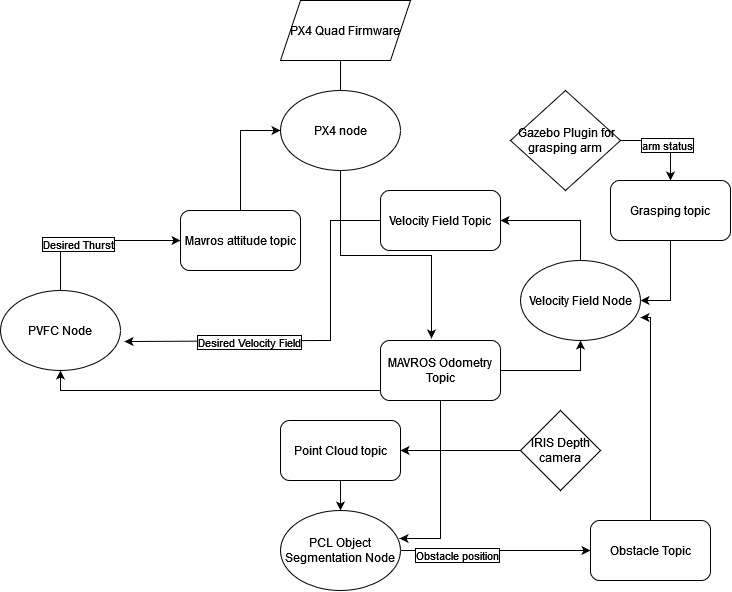
\includegraphics[width=\linewidth]{Images/implementation diagram.jpg}
    \caption{implementation diagram}
    \label{fig:implementationdiagram}
\end{figure*}

